%% ============================================================
%%  docs/octree.tex
%%  Scientific article: Adaptive SDF Octrees for Real-Time
%%  Terrain CSG and Surface Nets Meshing
%% ============================================================
\documentclass[10pt,a4paper]{article}

\usepackage[T1]{fontenc}
\usepackage[utf8]{inputenc}
\usepackage{lmodern}
\usepackage{microtype}
\usepackage{geometry}
\geometry{left=2.5cm, right=2.5cm, top=2.8cm, bottom=2.8cm}

\usepackage{amsmath,amssymb,amsthm}
\DeclareMathOperator*{\argmin}{arg\,min}
\usepackage{xcolor}
\usepackage{graphicx}
\usepackage{booktabs}
\usepackage{hyperref}
\usepackage{cleveref}
\usepackage{float}
\usepackage{caption}
\usepackage{subcaption}
\usepackage{enumitem}
\usepackage{multicol}

%% ---- TikZ ---------------------------------------------------
\usepackage{tikz}
\usetikzlibrary{
  arrows.meta, positioning, shapes.geometric, fit, calc,
  decorations.pathreplacing, backgrounds, patterns
}
\usepackage{pgfplots}
\pgfplotsset{compat=1.18}

%% ---- Algorithms --------------------------------------------
\usepackage{algorithm}
\usepackage{algpseudocode}

%% ---- Listings ----------------------------------------------
\usepackage{listings}
\lstdefinestyle{cpp}{
  language=C++,
  basicstyle=\ttfamily\small,
  keywordstyle=\color{blue!70!black}\bfseries,
  commentstyle=\color{gray!60},
  stringstyle=\color{orange!80!black},
  numberstyle=\tiny\color{gray},
  numbers=left,
  numbersep=6pt,
  breaklines=true,
  tabsize=2,
  showstringspaces=false,
  frame=single,
  rulecolor=\color{gray!30},
  backgroundcolor=\color{gray!4},
  captionpos=b
}
\lstset{style=cpp}

%% ---- Theorem environments ----------------------------------
\newtheorem{definition}{Definition}
\newtheorem{remark}{Remark}

%% ---- TikZ helpers ------------------------------------------
% Oblique-projection helper: (x,y,z) -> 2D with z into page
% proj_x = x + 0.40*z,  proj_y = y + 0.30*z
\newcommand{\prjnode}[4]{% \prjnode{name}{x}{y}{z}
  \pgfmathsetmacro{\px}{#2 + 0.40*(#4)}
  \pgfmathsetmacro{\py}{#3 + 0.30*(#4)}
  \coordinate (#1) at (\px, \py);
}

%% ============================================================
\title{%
  \textbf{Adaptive SDF Octrees for Real-Time Terrain CSG and Surface Nets Meshing}\\[4pt]
  {\large Structure, Operations, and Triangle Extraction}
}
\author{Vulkan Engine Technical Report}
\date{2026}

\begin{document}
\maketitle

\begin{abstract}
We describe the design and implementation of an adaptive octree that
serves as the primary spatial data structure for real-time constructive
solid geometry (CSG) on signed distance function (SDF)-defined terrain.
The octree stores per-corner SDF samples at each node, enabling
efficient region classification (\emph{Empty}, \emph{Solid},
\emph{Surface}), dynamic CSG through a recursive \emph{shape} pass, and
LOD-aware simplification.  Mesh extraction uses a \emph{surface nets}
algorithm: for every axis-aligned edge crossing the SDF zero-surface, a
dual polygon is assembled from the four cells sharing that edge.  An
ownership rule prevents duplicate emission across cell boundaries, and
winding is determined authoritatively from the SDF sign at the edge
endpoints.  The resulting mesh is directly fed to a Vulkan renderer
operating under $\texttt{VK\_FRONT\_FACE\_CLOCKWISE}$ convention.  This
report provides a complete, self-contained technical reference targeted at
graphics-engine developers.
\end{abstract}

\tableofcontents
\newpage

% ============================================================
\section{Introduction}
\label{sec:intro}
% ============================================================

Implicit surfaces defined by signed distance functions are an
increasingly popular representation for procedurally generated terrain,
sculpted worlds, and destructible environments in real-time applications.
A SDF assigns a real-valued \emph{distance} to every point in space: its
sign encodes whether the point lies inside or outside the solid, and its
magnitude gives the closest distance to the surface.  Because SDFs compose
cleanly under boolean operations and can be evaluated anywhere in constant
time, they are ideally suited to constructive solid geometry (CSG)
workflows.

Converting an implicit surface to a triangle mesh, however, requires
explicitly locating the zero iso-surface.  Classic algorithms such as
Marching Cubes~\cite{lorensen87} operate on regular grids, which scales
poorly for large terrain at high resolution.  Adaptive octrees address
this by concentrating detail only where the surface passes, giving
$\mathcal{O}(N)$ storage proportional to the surface area rather than the
volume.

The system described in this report uses a \emph{surface nets} approach
(a variant of \emph{dual contouring}~\cite{ju02}) combined with a
single-pass \emph{shape} traversal that evaluates CSG operations and
updates the octree incrementally.  The key technical contributions are:
\begin{enumerate}
  \item A compact node representation storing eight per-corner SDF samples
    together with a simplified surface vertex.
  \item A recursive CSG pass (\S\ref{sec:shape}) with optional
    multi-threaded subtree evaluation and angle/distance-based
    simplification.
  \item An edge-centric mesh extractor (\S\ref{sec:itriangles}) that
    handles non-uniform LOD boundaries, resolves ownership unambiguously,
    and determines polygon winding from the SDF sign alone.
\end{enumerate}

\bigskip\noindent
The remainder of the report is structured as follows.
Section~\ref{sec:sdf} reviews SDFs.
Section~\ref{sec:octree} describes the octree data structure.
Section~\ref{sec:shape} details the CSG pass.
Section~\ref{sec:itriangles} explains surface nets extraction.
Section~\ref{sec:tesselator} covers UV mapping.
Section~\ref{sec:discussion} discusses design trade-offs and limitations.

% ============================================================
\section{Signed Distance Functions}
\label{sec:sdf}
% ============================================================

\subsection{Definition}

\begin{definition}[Signed Distance Function]
A \emph{signed distance function} is a scalar field
$f:\mathbb{R}^3\to\mathbb{R}$ satisfying
\[
  f(\mathbf{p}) = s(\mathbf{p})\,\inf_{\mathbf{q}\in\partial\Omega}
    \|\mathbf{p}-\mathbf{q}\|,
\]
where $\partial\Omega$ is the surface and $s(\mathbf{p})\in\{-1,+1\}$
is the sign: $-1$ if $\mathbf{p}$ is inside the solid, $+1$ outside.
\end{definition}

\noindent The convention used throughout the codebase is:
\[
  f(\mathbf{p}) < 0 \;\Longrightarrow\; \mathbf{p}\in\Omega\text{ (solid)},
  \qquad
  f(\mathbf{p}) > 0 \;\Longrightarrow\; \mathbf{p}\notin\Omega\text{ (empty)}.
\]
The surface is the zero level set $\{f=0\}$.  An important property of
true SDFs is $\|\nabla f\| = 1$ almost everywhere
(\emph{eikonal equation}); however, the CSG operations described below
do not always preserve this property exactly, and the system uses the
gradient only for surface-normal estimation, where a unit-norm gradient
is normalised explicitly.

\subsection{Boolean CSG Operations}
\label{sec:sdf:ops}

The following boolean operations are implemented (Figure~\ref{fig:sdf_ops}):

\begin{center}
\begin{tabular}{lll}
  \toprule
  Operation & Formula & Description\\
  \midrule
  Union        & $\min(f_1, f_2)$              & Fill-in of two solids \\
  Subtraction  & $\max(f_1, -f_2)$             & Carve $\Omega_2$ from $\Omega_1$\\
  Intersection & $\max(f_1, f_2)$              & Keep only overlap \\
  Smooth union & $\text{smin}(f_1,f_2,k)$      & Union with blending radius $k$\\
  Smooth sub.  & $\text{ssub}(f_1,f_2,k)$      & Subtraction with rounding\\
  Paint        & $\min(f_1,\max(f_1,f_2))$     & Material override, shape unchanged\\
  \bottomrule
\end{tabular}
\end{center}

The smooth union is the standard Inigo Quilez exponential blend:
\[
  h = \text{clamp}\!\left(0.5 + \tfrac{f_2-f_1}{2k},\,0,\,1\right),
  \quad
  \text{smin}(f_1,f_2,k) = \text{lerp}(f_2,f_1,h) - k\,h\,(1-h).
\]
Setting $k=0$ recovers the hard union.  The \emph{paint} operation has
no geometric effect: $\min(d_1,\max(d_1,d_2)) = d_1$ when $d_1 < d_2$
and $d_2$ when $d_1 \geq d_2$.  It is used to repaint material indices
without altering shape.

\begin{figure}[htb]
\centering
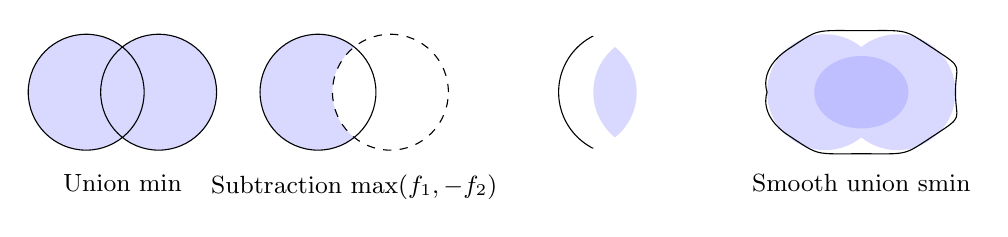
\begin{tikzpicture}[scale=0.92]
  % Union: circles A and B, filled interior
  \begin{scope}[shift={(0,0)}]
    \fill[blue!15] (0,0) circle (0.8);
    \fill[blue!15] (1.0,0) circle (0.8);
    \draw (0,0) circle (0.8);
    \draw (1.0,0) circle (0.8);
    \node[below, font=\small] at (0.5,-1.0) {Union $\min$};
  \end{scope}
  % Subtraction: A minus B
  \begin{scope}[shift={(3.2,0)}]
    \fill[blue!15] (0,0) circle (0.8);
    \fill[white]   (1.0,0) circle (0.8);
    \draw (0,0) circle (0.8);
    \draw[dashed] (1.0,0) circle (0.8);
    \node[below, font=\small] at (0.5,-1.0) {Subtraction $\max(f_1,-f_2)$};
  \end{scope}
  % Intersection: only overlap
  \begin{scope}[shift={(6.8,0)}]
    \clip (0,0) circle (0.8);
    \fill[blue!15] (1.0,0) circle (0.8);
    \begin{scope}[reset cm]
      \draw[shift={(6.8,0)}] (0,0) circle (0.8);
      \draw[shift={(6.8,0)}, dashed] (1.0,0) circle (0.8);
    \end{scope}
    \node[below, font=\small] at (0.5,-1.0) {Intersection $\max$};
  \end{scope}
  % Smooth union: blended boundary
  \begin{scope}[shift={(10.2,0)}]
    \fill[blue!15] (0,0) circle (0.8);
    \fill[blue!15] (1.0,0) circle (0.8);
    \fill[blue!25] (0.5,0) ellipse (0.65 and 0.5);
    \draw plot[smooth, tension=1.2] coordinates {(-0.8,0) (-0.5,-0.6) (0.5,-0.85) (1.5,-0.6) (1.8,0) (1.5,0.6) (0.5,0.85) (-0.5,0.6) (-0.8,0)};
    \node[below, font=\small] at (0.5,-1.0) {Smooth union $\text{smin}$};
  \end{scope}
\end{tikzpicture}
\caption{2D cross-section of four CSG operations.  Blue fill indicates the solid
region $\{f<0\}$.}
\label{fig:sdf_ops}
\end{figure}

\subsection{Per-Corner Sampling and Trilinear Interpolation}
\label{sec:sdf:corners}

The octree stores the SDF at each of the eight corners of an
axis-aligned bounding cube.  Let the cube have minimum corner $\mathbf{m}$
and side length $\ell$; then the value at corner $i$ is
\[
  d_i = f\!\left(\mathbf{m} + \ell\,\mathbf{s}_i\right),
  \qquad
  \mathbf{s}_i = \bigl(\tfrac{i_x}{1}, \tfrac{i_y}{1}, \tfrac{i_z}{1}\bigr)
    \in \{0,1\}^3,
\]
where $(i_x, i_y, i_z)$ are the bits of $i$ (see \S\ref{sec:octree:corners}).
Given the eight samples $d_0,\ldots,d_7$, an \emph{interior} value is
recovered by trilinear interpolation:
\[
  f_{\text{tri}}(\mathbf{p}) =
    \sum_{k=0}^{7}
      d_k\;
      \lambda_{k_x}(t_x)\,
      \lambda_{k_y}(t_y)\,
      \lambda_{k_z}(t_z),
  \qquad
  \lambda_0(\alpha) = 1-\alpha,\quad
  \lambda_1(\alpha) = \alpha,
\]
where $\mathbf{t} = (\mathbf{p}-\mathbf{m})/\ell\in[0,1]^3$.

\subsection{Surface-Normal Estimation}
\label{sec:sdf:normal}

The outward normal at any point $\mathbf{p}$ inside a node's cube is
estimated as the normalised gradient of $f_{\text{tri}}$:
\[
  \hat{\mathbf{n}}(\mathbf{p}) =
    \frac{\nabla f_{\text{tri}}(\mathbf{p})}
         {\|\nabla f_{\text{tri}}(\mathbf{p})\|}.
\]
The gradient components are computed analytically from the trilinear
formula using the chain rule, yielding a per-axis formula that sums
differences of opposite-face corner values weighted by the barycentric
coordinates in the other two directions:
\begin{align*}
  \partial_x f &= \frac{1}{\ell}\Bigl[
    (1-t_y)(1-t_z)(d_4-d_0) + t_y(1-t_z)(d_6-d_2) +
    (1-t_y)t_z(d_5-d_1) + t_y t_z(d_7-d_3)
  \Bigr],
\end{align*}
with analogous expressions for $\partial_y f$ and $\partial_z f$.  This
normal is stored as \lstinline{Vertex::normal} and is used for both
lighting and surface-normal-based winding heuristics.

\subsection{Vertex Placement via QEF}
\label{sec:sdf:qef}

Within each surface node, the \emph{representative vertex} is placed at
the minimiser of a Quadratic Error Function (QEF) that enforces alignment
with the local surface.  For each of the 12 edges $e$ of the cube with a
sign change, let $\mathbf{p}_e$ be the edge crossing (found by linear
interpolation) and $\hat{\mathbf{n}}_e$ the interpolated normal there.
The QEF minimises
\[
  E(\mathbf{x}) = \sum_e \bigl(\hat{\mathbf{n}}_e \cdot \mathbf{x} - d_e\bigr)^2,
  \qquad d_e = \hat{\mathbf{n}}_e \cdot \mathbf{p}_e,
\]
leading to the least-squares linear system $A^\top\!A\,\mathbf{x} = A^\top b$ where
$A^\top\!A = \sum_e \hat{\mathbf{n}}_e\hat{\mathbf{n}}_e^\top$ and
$A^\top b = \sum_e d_e\hat{\mathbf{n}}_e$.  When the matrix is
sufficiently well-conditioned ($|\det(A^\top\!A)| > \epsilon$), the
unique minimiser is computed; otherwise, the system falls back to the
centroid of the sign-change midpoints (\lstinline{getAveragePosition}).

\subsection{Primitive Catalogue}

The engine provides a library of analytic primitives:

\begin{center}
\begin{tabular}{lll}
  \toprule
  Primitive & Key parameter(s) & SDF formula (sketch)\\
  \midrule
  Box          & half-extents $\mathbf{b}$ & $\|\max(|\mathbf{p}|-\mathbf{b},0)\| + \min(\max(\ldots),0)$\\
  Sphere/Capsule & radius $r$            & $\|\mathbf{p}\| - r$, segment variant\\
  Cylinder     & radius $r$, height $h$  & 2D annulus + height clamp\\
  Torus        & major $R$, minor $r$    & $\|\,(|\mathbf{p}.xz|-R,\mathbf{p}.y)\| - r$\\
  Height-map   & DEM raster              & lookup + trilinear interpolation\\
  Perlin noise & amplitude, frequency    & layered stb\_perlin noise field\\
  Voronoi 3D   & cell size, seed         & domain-warped Voronoi distance\\
  Triangle strip& 4 verts, half-thickness& min of two extruded-triangle SDFs\\
  \bottomrule
\end{tabular}
\end{center}

Composite shapes are built by wrapping primitives in a
\lstinline{WrappedSignedDistanceFunction} and combining them with a
binary operation (Table in \S\ref{sec:sdf:ops}).

% ============================================================
\section{Adaptive Octree Data Structure}
\label{sec:octree}
% ============================================================

\subsection{Corner Indexing Convention}
\label{sec:octree:corners}

Each internal or leaf node owns an axis-aligned cube.  The cube has eight
corners indexed $0,\ldots,7$ by a three-bit field:
\begin{equation}
  \label{eq:corner_index}
  \text{idx}(\mathbf{p}) =
    \underbrace{[x \geq c_x]}_{\text{bit 2}} \cdot 4 \;+\;
    \underbrace{[y \geq c_y]}_{\text{bit 1}} \cdot 2 \;+\;
    \underbrace{[z \geq c_z]}_{\text{bit 0}} \cdot 1,
\end{equation}
where $\mathbf{c} = (c_x,c_y,c_z)$ is the cube centre and $[\cdot]$
is the Iverson bracket.  The coordinates of each corner are therefore:

\begin{center}
\begin{tabular}{c|c|c|c|c}
  \toprule
  Index & $x$ & $y$ & $z$ & Bit pattern (xyz)\\
  \midrule
  0 & min & min & min & 000 \\
  1 & min & min & max & 001 \\
  2 & min & max & min & 010 \\
  3 & min & max & max & 011 \\
  4 & max & min & min & 100 \\
  5 & max & min & max & 101 \\
  6 & max & max & min & 110 \\
  7 & max & max & max & 111 \\
  \bottomrule
\end{tabular}
\end{center}

Figure~\ref{fig:cube_corners} illustrates the layout.  Note the
relationship: flipping bit $k$ of an index transitions to the
corner that is adjacent along axis $k$.  For instance,
corner 3 (011) and corner 7 (111) differ only in bit 2, so they are
connected by an edge along the $x$-axis.

\begin{figure}[htb]
\centering
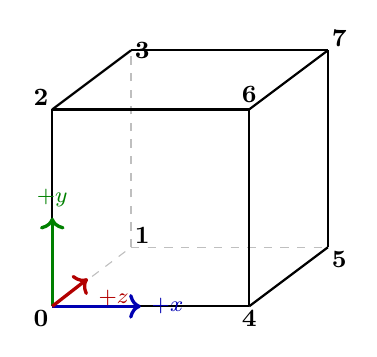
\begin{tikzpicture}[scale=2.5, thick, font=\small]
  % Oblique projection: (x,y,z) -> (x + 0.40z, y + 0.30z)
  % Scale: unit cube = 1 TikZ unit = 2.5 cm
  \coordinate (C0) at (0.00, 0.00);  % (0,0,0)
  \coordinate (C1) at (0.40, 0.30);  % (0,0,1)
  \coordinate (C2) at (0.00, 1.00);  % (0,1,0)
  \coordinate (C3) at (0.40, 1.30);  % (0,1,1)
  \coordinate (C4) at (1.00, 0.00);  % (1,0,0)
  \coordinate (C5) at (1.40, 0.30);  % (1,0,1)
  \coordinate (C6) at (1.00, 1.00);  % (1,1,0)
  \coordinate (C7) at (1.40, 1.30);  % (1,1,1)

  % Hidden edges (dashed)
  \draw[gray!50, dashed, thin] (C0) -- (C1);
  \draw[gray!50, dashed, thin] (C1) -- (C3);
  \draw[gray!50, dashed, thin] (C1) -- (C5);

  % Visible edges
  \draw (C0) -- (C4);   % bottom front
  \draw (C0) -- (C2);   % left front
  \draw (C4) -- (C6);   % right front
  \draw (C2) -- (C6);   % top front
  \draw (C4) -- (C5);   % bottom right depth
  \draw (C5) -- (C7);   % right side back
  \draw (C6) -- (C7);   % top right depth
  \draw (C2) -- (C3);   % top left depth
  \draw (C3) -- (C7);   % top back

  % Corner labels
  \node[below left, inner sep=1pt]  at (C0) {$\mathbf{0}$};
  \node[above right, inner sep=1pt] at (C1) {$\mathbf{1}$};
  \node[above left, inner sep=1pt]  at (C2) {$\mathbf{2}$};
  \node[right, inner sep=1pt]       at (C3) {$\mathbf{3}$};
  \node[below, inner sep=1pt]       at (C4) {$\mathbf{4}$};
  \node[below right, inner sep=1pt] at (C5) {$\mathbf{5}$};
  \node[above, inner sep=2pt]       at (C6) {$\mathbf{6}$};
  \node[above right, inner sep=1pt] at (C7) {$\mathbf{7}$};

  % Axis arrows
  \draw[->, blue!70!black, very thick]
    (C0) -- ++(0.45,0) node[right, font=\footnotesize]{$+x$};
  \draw[->, green!50!black, very thick]
    (C0) -- ++(0,0.45) node[above, font=\footnotesize]{$+y$};
  \draw[->, red!70!black, very thick]
    (C0) -- ++(0.18, 0.14) node[below right, font=\footnotesize]{$+z$};
\end{tikzpicture}
\caption{Cube corner numbering.  Index bits: bit~2 = $x\geq c_x$,
bit~1 = $y\geq c_y$, bit~0 = $z\geq c_z$.
Dashed edges are hidden in this view.}
\label{fig:cube_corners}
\end{figure}

\subsection{The Twelve Cube Edges}
\label{sec:octree:edges}

The 12 axis-aligned edges of a cube are encoded as pairs of corner
indices:

\begin{center}
\small
\begin{tabular}{c|c|l}
  \toprule
  Edge index & Corner pair & Axis and fixed coords\\
  \midrule
  0  & $\{0,1\}$ & $z$-axis at $(x_{\min}, y_{\min})$\\
  1  & $\{1,3\}$ & $y$-axis at $(x_{\min}, z_{\max})$\\
  2  & $\{2,3\}$ & $z$-axis at $(x_{\min}, y_{\max})$\\
  3  & $\{0,2\}$ & $y$-axis at $(x_{\min}, z_{\min})$\\
  4  & $\{4,5\}$ & $z$-axis at $(x_{\max}, y_{\min})$\\
  5  & $\{5,7\}$ & $y$-axis at $(x_{\max}, z_{\max})$\\
  6  & $\{6,7\}$ & $z$-axis at $(x_{\max}, y_{\max})$\\
  7  & $\{4,6\}$ & $y$-axis at $(x_{\max}, z_{\min})$\\
  8  & $\{0,4\}$ & $x$-axis at $(y_{\min}, z_{\min})$\\
  9  & $\{1,5\}$ & $x$-axis at $(y_{\min}, z_{\max})$\\
  10 & $\{2,6\}$ & $x$-axis at $(y_{\max}, z_{\min})$\\
  11 & $\{3,7\}$ & $x$-axis at $(y_{\max}, z_{\max})$\\
  \bottomrule
\end{tabular}
\end{center}

\noindent
A sign change on edge $e$ (i.e.\ $d_{e_0} < 0 \neq d_{e_1} < 0$ or
vice versa) means the iso-surface crosses that edge, which is the
trigger for surface-net polygon emission (\S\ref{sec:itriangles}).

\subsection{Node Layout}

Each node in the octree (\lstinline{OctreeNode}) stores:
\begin{itemize}[leftmargin=2em]
  \item \lstinline{float sdf[8]} — SDF values sampled at the eight cube corners.
  \item \lstinline{Vertex vertex} — the representative surface vertex
    (position, normal, texture coordinate, brush/material index).
  \item \lstinline{uint blockId} — index into a slab allocator pointing
    to the \lstinline{ChildBlock} (8 child pointers), or null if leaf.
  \item \lstinline{uint8_t bits} — a compact bitfield encoding:
    \begin{itemize}
      \item \emph{SpaceType} (2 bits): \lstinline{Empty}/\lstinline{Solid}/\lstinline{Surface}.
      \item \emph{Simplified} (1 bit): set when the node's children have been
        merged into this coarser representation.
      \item \emph{Chunk} (1 bit): marks the root of a GPU upload chunk.
      \item \emph{Leaf} (1 bit): no children exist.
    \end{itemize}
  \item \lstinline{uint version} — incremented when a chunk's geometry
    changes, used for cache invalidation.
\end{itemize}

\subsection{SpaceType Classification}
\label{sec:octree:spacetype}

Each node is classified into one of three types by inspecting
$d_0,\ldots,d_7$:
\begin{align*}
  \text{Solid}   &: \forall i,\; d_i < 0\phantom{\text{ and }\exists j} \\
  \text{Empty}   &: \forall i,\; d_i \geq 0\\
  \text{Surface} &: \exists\, i,j \text{ s.t.\ } d_i < 0 \text{ and } d_j \geq 0
\end{align*}
(treating $\infty$ as ``untouched'', excluded from both tests).
Only \lstinline{Surface} nodes carry a representative vertex and
participate in mesh extraction.  Solid and Empty nodes are pruned of
children once the subtree below them is fully classified, keeping memory
usage proportional to the surface area.

\subsection{Memory Model}

Nodes are managed through a pool allocator (\lstinline{OctreeAllocator}),
which maintains two slab arenas: one for \lstinline{OctreeNode} instances
and one for \lstinline{ChildBlock}s (arrays of 8 child pointers).
The pool design eliminates per-node heap overhead and allows the entire
octree to be reset in $O(1)$.  Deferred GPU-safe destruction is handled
by fencing rather than immediate freeing.

\subsection{Chunk and Thread Hierarchy}

The octree hierarchy has two special levels:
\begin{description}
  \item[Chunk nodes] Nodes whose cube side length $\ell$ satisfies
    $0.5\ell_{\mathrm{chunk}} < \ell \leq \ell_{\mathrm{chunk}}$.
    They are not simplified (their children remain expanded), and each
    triggers an \lstinline{onNodeAdded}/\lstinline{onNodeDeleted}
    callback that schedules a GPU geometry upload.
  \item[Thread nodes] Nodes whose cube is large enough
    ($\ell > \ell_{\min} \cdot 16$) spawn subtree evaluations on a
    shared thread pool.  Each thread works within its own
    \lstinline{ThreadContext} (per-thread caches for SDF values and
    visited nodes) to avoid contention.
\end{description}

% ============================================================
\section{CSG Operations: \texttt{apply}, \texttt{expand}, and \texttt{shape}}
\label{sec:shape}
% ============================================================

The entry point for CSG is \lstinline{Octree::apply}, which wraps all
modification steps: dynamic expansion, recursive descent, and GPU upload
scheduling.  The call graph is:

\begin{center}
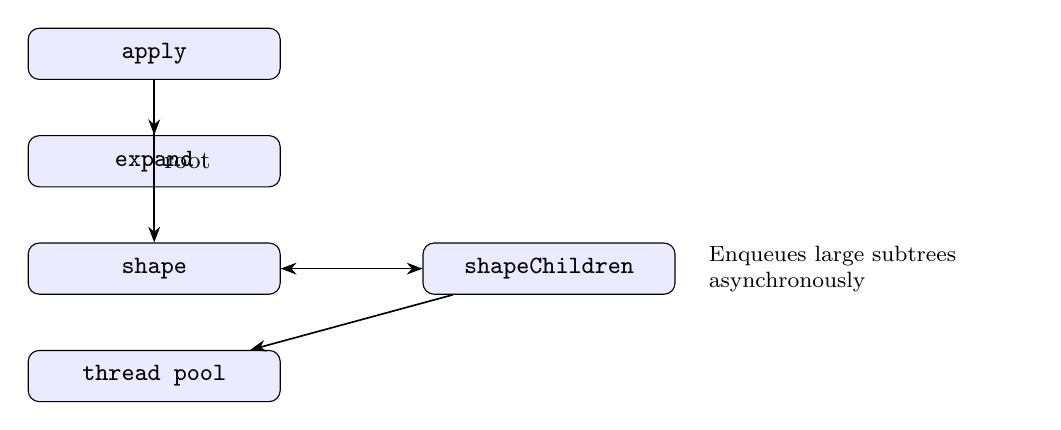
\begin{tikzpicture}[
    box/.style={draw, rounded corners, fill=blue!8,
                minimum width=3.2cm, minimum height=0.65cm,
                font=\small\ttfamily},
    arr/.style={->, >=Stealth, semithick}
  ]
  \node[box] (apply)   {\textbf{apply}};
  \node[box, below=0.7cm of apply]  (expand) {expand};
  \node[box, below=0.7cm of expand] (shape)  {shape};
  \node[box, right=1.8cm of shape]  (shapeC) {shapeChildren};
  \node[box, below=0.7cm of shape]  (thread) {thread pool};
  \draw[arr] (apply) -- (expand);
  \draw[arr] (apply) -- node[right, font=\small]{root} (shape);
  \draw[arr, bend right=25] (shape) -- (shapeC);
  \draw[arr, bend right=25] (shapeC) -- (shape);
  \draw[arr] (shapeC) -- (thread);
  \node[draw=none, right=0.3cm of shapeC, font=\footnotesize,
        text width=4cm, align=left]
    {Enqueues large subtrees\\asynchronously};
\end{tikzpicture}
\end{center}

\subsection{Dynamic Expansion (\texttt{expand})}

The octree root may not initially contain the entire SDF domain.
\lstinline{expand} grows the tree by repeatedly doubling the world cube
until \lstinline{function->isContained} returns true.  Each doubling:
\begin{enumerate}
  \item Computes which octant of the new (doubled) cube the old root
    occupies (using the SDF centroid to choose the complementary octant
    index: \lstinline{i ^ 0x7}).
  \item Allocates a new root node and a new \lstinline{ChildBlock}, then
    places the old root as child $i$.
  \item Updates the stored bounds (\lstinline{min}, \lstinline{length}).
\end{enumerate}
This operation is idempotent and fast: it performs only $O(\log R)$ node
allocations for an expansion factor $R$.

\subsection{Recursive Descent (\texttt{shape})}
\label{sec:shape:shape}

\lstinline{shape} is the central recursive function.  Given a node frame
$(\textit{node}, \textit{cube}, \textit{level}, \textit{sdf}[8],
\textit{brushIndex})$, it:

\begin{algorithm}[H]
\caption{\lstinline{shape}(frame, args)}
\label{alg:shape}
\begin{algorithmic}[1]
\State $\text{shapeSDF} \leftarrow \text{evaluateShapeSDF}(\text{frame})$
\If{$\text{frame.isLeaf}$}
  \State $\text{resultSDF} \leftarrow \text{args.operation}(\text{frame.sdf}, \text{shapeSDF})$
  \State classify $\text{resultType}$
\Else
  \If{$\text{args.function.check(cube)} = \text{Disjoint}$}
    \State $\text{resultSDF} \leftarrow \text{frame.sdf}$ \Comment{no-op, shape does not reach this cube}
  \Else
    \State $\text{shapeChildren}(\text{frame})$ \Comment{recurse on all 8 children}
    \State aggregate child types $\to$ $\text{resultType}$
  \EndIf
\EndIf
\If{$\text{resultType} = \text{Surface}$}
  \State allocate node if needed
  \State $\text{node.vertex.position} \leftarrow \text{getAveragePosition}(\text{resultSDF})$
  \State $\text{node.vertex.normal} \leftarrow \nabla f(\text{position})$
  \If{$\text{isLeaf}$}
    \State $\text{brushIndex} \leftarrow \text{painter.paint}(\text{vertex})$
  \Else
    \State attempt $\text{simplification}$ (\S\ref{sec:shape:simplify})
    \State link children into node's \lstinline{ChildBlock}
  \EndIf
\EndIf
\State write $\text{resultType}$, $\text{resultSDF}$, $\text{isSimplified}$, $\text{brushIndex}$ into node
\If{$\text{isChunk}$ and $\text{resultType} = \text{Surface}$}
  \State fire \lstinline{onNodeAdded} callback (GPU upload)
\EndIf
\end{algorithmic}
\end{algorithm}

\paragraph{SDF composition.}
At each node, the shape's SDF is evaluated at the 8 cube corners via the
\lstinline{WrappedSignedDistanceFunction::distance} interface (with an
optional corner-level cache).  The result is then composed with the
current node's SDF using the user-supplied binary operation:
\[
  d_i^{\text{result}} = \text{op}(d_i^{\text{current}},\; d_i^{\text{shape}}).
\]

\paragraph{Child SDF propagation.}
When a child node does not yet exist, its 8 corner SDF values must be
derived from the parent.  This is done by
\lstinline{SDF::getChildSDF}: the eight corners of the child cube (which
lie within the parent cube) are interpolated from the parent's
$d_0,\ldots,d_7$ via trilinear interpolation on a canonical unit cube.
This avoids re-evaluating the potentially expensive SDF primitive.

\paragraph{Node allocation.}
If a surface result is computed for a position where no node exists
(e.g.\ when a new brush stroke creates a previously empty region), a new
\lstinline{OctreeNode} is allocated from the pool, initialised with the
cube centre as its temporary vertex position, and refined with the QEF
minimiser.

\subsection{Simplification}
\label{sec:shape:simplify}

After all eight children have been processed, the
\lstinline{Simplifier::simplify} routine attempts to merge them into the
parent node.  The test has three conditions, each of which can veto
simplification:

\begin{enumerate}
  \item \textbf{Texture uniformity.} If texturing is enabled, all surface
    children must carry the same brush index.  Any texture boundary blocks
    simplification to preserve material edges.
  \item \textbf{All-simplified children.} Every surface child must itself
    be simplified (i.e.\ recursively merged below it).
  \item \textbf{SDF error bound.} For each surface child, the
    \emph{re-interpolated} parent SDF (evaluated at the child's corners
    from the parent's $d_0,\ldots,d_7$) is compared against the child's
    actual SDF.  If the pointwise error exceeds
    $10\%$ of the parent cube side length:
    \[
      |d_{\text{parent-interp}}(c_j) - d_{\text{child}}(c_j)| >
        0.1\,\ell_{\text{parent}},
    \]
    the child geometry is too detailed to represent faithfully at coarser
    resolution, and simplification is rejected.
\end{enumerate}

\noindent
If simplification succeeds, the parent node's \emph{simplified} bit is
set, the child nodes are retained in the tree but their geometry is
\emph{represented} by the parent for rendering purposes.  Chunk-boundary
nodes are never simplified to preserve consistent GPU upload granularity.

\subsection{Parallelism}

When \lstinline{shapeChildren} encounters a child whose cube side length
exceeds $16 \cdot \ell_{\min}$, the child's subtree is enqueued on a
\lstinline{ThreadPool} backed by \lstinline{std::thread::hardware_concurrency}
threads.  Each worker receives its own \lstinline{ThreadContext} which
holds:
\begin{itemize}
  \item A per-subtree \lstinline{robin_map} cache for SDF evaluations
    (avoids redundant primitive distance computations within a subtree).
  \item A per-subtree node-level cache for \lstinline{getNodeAt} lookups.
\end{itemize}
Parent-level coordination happens via \lstinline{std::future}: after
dispatching all eight potential threads, the parent waits on all futures
before aggregating child results.

% ============================================================
\section{Surface Nets Mesh Extraction: \texttt{iterateTriangles}}
\label{sec:itriangles}
% ============================================================

\subsection{Overview and Comparison with Marching Cubes}

\emph{Marching Cubes}~\cite{lorensen87} is a \emph{primal} method: for
each cell that straddles the surface it emits a triangle by looking up a
precomputed table of 15 topological cases based on the 8 corner signs.
The vertices lie on cell edges.  The method is simple and robust but
produces blocky meshes (staircase artefacts) and cannot naturally handle
multiple cells sharing one edge at different LOD levels.

\emph{Dual contouring}~\cite{ju02} and \emph{surface nets}~\cite{gibson98}
are \emph{dual} methods.  Rather than placing vertices on edges, they
place one vertex \emph{inside} each surface cell and connect neighbouring
vertices through faces shared between cells.  The key advantage is that
vertex positions can be optimised (via QEF) to reproduce sharp
features.  The implementation here uses the surface-nets formulation:

\begin{quote}
  \emph{For each axis-aligned edge that crosses the surface, emit one
  polygon whose corners are the representative vertices of the four
  cells surrounding that edge.}
\end{quote}

\noindent The result is a closed, manifold mesh (under correct winding) that
adapts naturally to the octree LOD without any explicit crack-filling.

\subsection{Edge Iteration and Sign-Change Detection}

\lstinline{iterateTriangles(from, fromCube, handler)} is called once for
every simplified surface node \lstinline{from}.  It iterates over all 12
edges of \lstinline{fromCube}.  For edge $e = \{e_0, e_1\}$, a sign
change is detected by:
\[
  \text{signChange}(e) \iff
    (d_{e_0} < 0) \neq (d_{e_1} < 0),
  \quad
  d_{e_k} = \texttt{from->sdf}[e_k].
\]
Only edges with a sign change are processed; the remaining 12 minus
those are skipped immediately.

\subsection{Edge Segmentation at LOD Boundaries}
\label{sec:itriangles:segseg}

In a uniform grid every edge has exactly two abutting cells per
transverse direction, giving four cells total.  In an adaptive octree,
neighbouring cells may exist at different LOD levels: a fine cell's edge
may overlap with a coarse cell's edge only partially.  Each edge must
therefore be split into sub-segments, one per contiguous region of
uniform cell coverage.

\begin{figure}[htb]
\centering
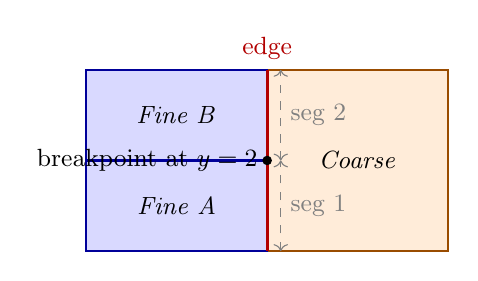
\begin{tikzpicture}[scale=1.15, font=\small]
  % Fine cells on the left, coarse cells on the right
  % The horizontal line is the shared edge (along x-axis)
  % Cells are in the y-direction

  % Coarse cell (spans full height on right side)
  \fill[orange!15] (0,1) rectangle (2,3);
  \draw[orange!60!black, thick] (0,1) rectangle (2,3);
  \node at (1, 2) {\textit{Coarse}};

  % Two fine cells on left side
  \fill[blue!15] (-2,1) rectangle (0,2);
  \draw[blue!60!black, thick] (-2,1) rectangle (0,2);
  \node at (-1, 1.5) {\textit{Fine A}};

  \fill[blue!15] (-2,2) rectangle (0,3);
  \draw[blue!60!black, thick] (-2,2) rectangle (0,3);
  \node at (-1, 2.5) {\textit{Fine B}};

  % The shared edge (x=0) from y=1 to y=3
  \draw[very thick, red!70!black] (0,1) -- (0,3)
    node[above, red!70!black] {edge};

  % Breakpoint annotation
  \draw[<->, dashed, black!50] (0.15,1) -- (0.15,2)
    node[midway, right] {seg 1};
  \draw[<->, dashed, black!50] (0.15,2) -- (0.15,3)
    node[midway, right] {seg 2};

  % Breakpoint dot
  \fill[black] (0,2) circle (1.5pt) node[left]{breakpoint at $y=2$};
\end{tikzpicture}
\caption{LOD boundary along an axis-aligned edge.  The edge (red) is shared
by two fine cells on one side and one coarse cell on the other.
\texttt{collectBreaks} inserts the cell-boundary at $y=2$ as a breakpoint,
splitting the edge into two sub-segments, each of which produces an
independent polygon.}
\label{fig:lod_boundary}
\end{figure}

\lstinline{collectBreaks} is a recursive procedure that inserts
breakpoints at all cell-boundary coordinates along the edge
(Algorithm~\ref{alg:breaks}).  It works by sampling a midpoint along the
current interval, querying the four surrounding cells, and extracting
their bounding cube min/max along the edge axis.  Any boundary coordinate
that falls strictly inside the interval and is not already in the list is
added.  The procedure then recurses on each sub-interval, halting at
depth~64 or when the interval is smaller than $2\varepsilon$.

\begin{algorithm}[H]
\caption{\lstinline{collectBreaks}(edge, start, end, breaks)}
\label{alg:breaks}
\begin{algorithmic}[1]
\If{$\text{depth} > 64$ \textbf{or} $\text{end} - \text{start} \leq 2\varepsilon$}
  \Return
\EndIf
\State $\text{mid} \leftarrow \tfrac{\text{start}+\text{end}}{2}$
\For{$q \in \{0,1,2,3\}$}
  \State $\text{cell} \leftarrow \text{findCellAt}(\text{quadrantSample}(\text{edge}, \text{mid}, q))$
  \State add $\text{cell.cube.min}[\text{axis}]$ and $\text{cell.cube.max}[\text{axis}]$ to breaks
\EndFor
\For{each sub-interval between adjacent breakpoints}
  \State $\text{collectBreaks}(\text{edge, sub.start, sub.end, breaks})$
\EndFor
\end{algorithmic}
\end{algorithm}

\subsection{Quadrant Sampling}
\label{sec:itriangles:quadrants}

Each sub-segment is processed by \lstinline{emitSegment}.  The four cells
surrounding the segment are found by querying the cell at a sample point
that is offset \emph{just inside} each quadrant around the edge axis.

Given an edge span with axis $a$ and fixed coordinates $(u_0, v_0)$ in
the two perpendicular axes, quadrant $q$ is sampled at:
\[
  \mathbf{p}_q = \bigl(t_{\text{mid}}, u_0 \oplus \varepsilon_u,\, v_0 \oplus \varepsilon_v\bigr)_a,
  \qquad (s_u, s_v) = \text{quadrantSigns}(a, q),
\]
where $t_{\text{mid}}$ is the segment midpoint along axis $a$,
$u_0 \oplus \varepsilon_u = \texttt{nextafter}(u_0,\pm\infty)$ depending
on $s_u$, and the quadrant signs follow the pattern shown in
Table~\ref{tab:quad_signs}.

\begin{table}[htb]
\centering
\caption{Quadrant sign table: $(s_u, s_v)$ for each axis and quadrant
index, defining the CCW ring when viewed from the positive axis direction.}
\label{tab:quad_signs}
\begin{tabular}{c|cccc}
\toprule
Axis & $q=0$ & $q=1$ & $q=2$ & $q=3$ \\
\midrule
$x$ (axes $u{=}y,\, v{=}z$) & $(-,-)$ & $(-,+)$ & $(+,+)$ & $(+,-)$\\
$y$ (axes $u{=}x,\, v{=}z$) & $(-,-)$ & $(+,-)$ & $(+,+)$ & $(-,+)$\\
$z$ (axes $u{=}x,\, v{=}y$) & $(-,-)$ & $(-,+)$ & $(+,+)$ & $(+,-)$\\
\bottomrule
\end{tabular}
\end{table}

The four quadrant cells are found by \lstinline{findCellAt}, which
descends the octree from the root to the deepest simplified surface
node that contains the sample point.  If any of the four cells is not
a surface node (or not simplified), the segment is silently skipped:
there is no surface to emit.

\begin{figure}[htb]
\centering
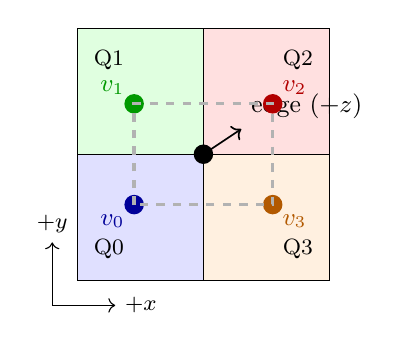
\begin{tikzpicture}[scale=1.6, font=\small]
  % Draw a 2x2 grid of cells sharing a central edge (along z axis, fixed x and y)
  % The edge is the vertical line at (0,0) going into the page; in this 2D view it's a dot

  % Cells: (u,v) quadrants around the edge point
  \fill[blue!10]  (-1,-1) rectangle (0,0);  % Q0: u-, v-
  \fill[green!10] (0,-1)  rectangle (1,0);  % Q1: u+, v- ... wait let me redo this
  % Actually for axis=z (into page), u=x and v=y.
  % Q0 = (x-, y-), Q1 = (x-, y+), Q2 = (x+, y+), Q3 = (x+, y-)
  % But the table says for axis=z: Q0=(-,-), Q1=(-,+), Q2=(+,+), Q3=(+,-)
  % So u=x, v=y:
  % Q0: x-, y-  Q1: x-, y+  Q2: x+, y+  Q3: x+, y-

  \fill[blue!12]  (-1,-1) rectangle (0,0);  % Q0: x-, y-
  \fill[green!12] (-1, 0) rectangle (0,1);  % Q1: x-, y+
  \fill[red!12]   (0,  0) rectangle (1,1);  % Q2: x+, y+
  \fill[orange!12](0, -1) rectangle (1,0);  % Q3: x+, y-

  % Cell boundaries
  \draw (-1,-1) rectangle (0,0);
  \draw (-1, 0) rectangle (0,1);
  \draw ( 0, 0) rectangle (1,1);
  \draw ( 0,-1) rectangle (1,0);

  % Central edge point (segment going into page)
  \fill[black] (0,0) circle (2.2pt);
  \draw[->, semithick] (0,0) -- (0.3, 0.2) node[above right]{edge ($+z$)};

  % Vertex positions (somewhere inside each cell)
  \fill[blue!60!black]  (-0.55, -0.4) circle (2.2pt) node[below left, blue!60!black]{$v_0$};
  \fill[green!60!black] (-0.55,  0.4) circle (2.2pt) node[above left, green!60!black]{$v_1$};
  \fill[red!70!black]   ( 0.55,  0.4) circle (2.2pt) node[above right, red!70!black]{$v_2$};
  \fill[orange!70!black]( 0.55, -0.4) circle (2.2pt) node[below right, orange!70!black]{$v_3$};

  % Polygon ring
  \draw[very thick, dashed, gray!60]
    (-0.55,-0.4) -- (-0.55,0.4) -- (0.55,0.4) -- (0.55,-0.4) -- cycle;

  % Quadrant labels
  \node at (-0.75, -0.75) {\footnotesize Q0};
  \node at (-0.75,  0.75) {\footnotesize Q1};
  \node at ( 0.75,  0.75) {\footnotesize Q2};
  \node at ( 0.75, -0.75) {\footnotesize Q3};

  % Axis labels
  \draw[->] (-1.2, -1.2) -- (-0.7, -1.2) node[right]{\footnotesize $+x$};
  \draw[->] (-1.2, -1.2) -- (-1.2, -0.7) node[above]{\footnotesize $+y$};
\end{tikzpicture}
\caption{Quadrant sampling for a $z$-axis edge (the dot at centre, going
into the page).  Four surrounding cells (one per quadrant) each
contribute one representative vertex $v_0,\ldots,v_3$.
The resulting polygon ring (dashed) forms the dual face.}
\label{fig:surface_nets_quad}
\end{figure}

\subsection{Ownership Rule}
\label{sec:itriangles:ownership}

When all four cells share the \emph{same} cell at the same LOD (a
uniform grid), any of them could claim responsibility for emitting the
polygon.  The ownership rule ensures each polygon is emitted exactly once
by designating the \emph{finest} (smallest) cell as the owner:

\begin{quote}
  $\text{owner} = \argmin_{q} \ell(\text{cell}_q)$,
  where ties are broken lexicographically by cube minimum corner, then by
  pointer address.
\end{quote}

\lstinline{emitSegment} compares the resolved owner against
\lstinline{from}.  If \lstinline{owner $\neq$ from}, the function returns
without emitting, deferring the polygon to the cell that \emph{is} the
finest.  This guarantees that the polygon is emitted exactly once per
underlying geometric boundary, regardless of how many times
\lstinline{iterateTriangles} is invoked (once per surface node).

\subsection{Polygon Ring Construction and Deduplication}
\label{sec:itriangles:dedup}

The four quadrant cells are inserted into the polygon array in quadrant
order ($q=0,1,2,3$).  Before insertion, two deduplication passes are
applied:

\begin{enumerate}
  \item \textbf{Adjacent-cell dedup.}  If the current cell is the same
    node (or has the same vertex position within $\varepsilon$) as the
    preceding entry, it is skipped.  This collapses consecutive identical
    cells at degenerate LOD boundaries.
  \item \textbf{Tail-head dedup.}  If the first and last entries refer to
    the same node (or coincident positions), the last entry is removed to
    avoid a degenerate closing edge.
  \item \textbf{All-pairs dedup.}  A final $O(n^2)$ check (over at most
    4 entries) discards the entire polygon if any two non-adjacent entries
    are identical, which would produce a self-intersecting or degenerate
    polygon.
\end{enumerate}

After deduplication, the polygon has 2, 3, or 4 entries.  Size~1 is
impossible after the all-pairs check.  Size~2 corresponds to a degenerate
edge (two collinear cells) and is silently dropped.

\paragraph{Rotation for reliable UV.}
After deduplication, the polygon is cyclically rotated so that
\lstinline{from} (the owner / finest cell) appears at index~0.  This is
necessary for UV mapping: the Tesselator uses
\lstinline{polygon[0].normal} for triplanar plane selection, and only
the finest cell's normal (computed from full-resolution SDF) is reliable
at curved LOD boundaries.

\subsection{Winding Determination from SDF Sign}
\label{sec:itriangles:winding}

Correct polygon orientation (so the front face is visible from outside
the solid) must be determined for every polygon.  Two naive approaches
fail:
\begin{description}
  \item[Geometric cross-product] Compute the cross product of two polygon
    edges and compare with the estimated surface normal.  Fails for
    \emph{non-planar quads}: at LOD boundaries four cells at different
    refinement levels generally do not form a planar quad; the two
    sub-triangles of the fan have cross products pointing in opposite
    directions, so a single flip decision gets one wrong.
  \item[Vertex-normal comparison] Compare $\hat{\mathbf{n}}_0$
    (the vertex normal of polygon[0]) with the geometric cross product.
    Fails when polygon[0] is a coarse neighbour cell whose normal is a
    broad average over a large region, potentially differing by $>90^\circ$
    from the true local surface direction.
\end{description}

The \emph{authoritative} approach is to derive winding directly from the
SDF sign change direction:

\begin{align*}
  d_0 &= f_{\text{tri}}(\mathbf{p}_{\text{start}},\;
          \text{owner.cube}), \\
  d_1 &= f_{\text{tri}}(\mathbf{p}_{\text{end}},\;
          \text{owner.cube}).
\end{align*}

The two endpoints $\mathbf{p}_{\text{start}}$ and $\mathbf{p}_{\text{end}}$
lie on the axis line at the start and end of the current sub-segment.
By construction, $\text{sign}(d_0) \neq \text{sign}(d_1)$.

\begin{figure}[htb]
\centering
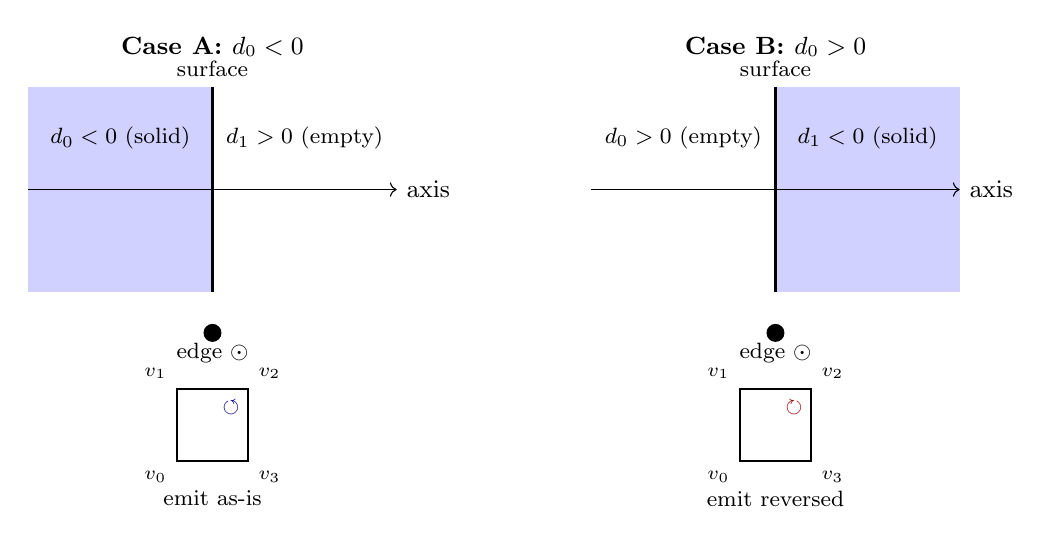
\begin{tikzpicture}[scale=1.3, font=\small]
  %--- Case 1: d0 < 0 (solid at start, surface faces +axis) ---
  \begin{scope}[shift={(0,0)}]
    % solid region (shaded)
    \fill[blue!18] (-1.8,-1.0) rectangle (0, 1.0);
    \fill[white]   (0,-1.0)    rectangle (1.8, 1.0);
    \draw[very thick] (0,-1.0) -- (0,1.0)
      node[above, font=\footnotesize]{surface};
    % axis arrow
    \draw[->] (-1.8,0) -- (1.8,0) node[right]{axis};
    % sign labels
    \node at (-0.9, 0.5) {\footnotesize $d_0 < 0$ (solid)};
    \node at ( 0.9, 0.5) {\footnotesize $d_1 > 0$ (empty)};
    % polygon ring in top-down view (circle = edge axis)
    \fill[black] (0,-1.4) circle (2.5pt);
    \node[below, font=\footnotesize] at (0,-1.4) {edge $\odot$};
    % CCW polygon v0..v3 around it (square)
    \begin{scope}[shift={(0,-2.3)}]
      \draw[thick, ->]
        (-0.35,-0.35) node[below left, font=\scriptsize]{$v_0$} --
        (-0.35, 0.35) node[above left, font=\scriptsize]{$v_1$} --
        ( 0.35, 0.35) node[above right, font=\scriptsize]{$v_2$} --
        ( 0.35,-0.35) node[below right, font=\scriptsize]{$v_3$} --
        cycle;
      \node[below, font=\footnotesize] at (0,-0.55) {emit as-is};
      \node[above right, font=\scriptsize, color=blue!60!black] at (0,0) {$\circlearrowleft$};
    \end{scope}
    % Case label
    \node[above, font=\bfseries\small] at (0, 1.2) {Case A: $d_0 < 0$};
  \end{scope}

  %--- Case 2: d0 > 0 (empty at start, surface faces -axis) ---
  \begin{scope}[shift={(5.5,0)}]
    \fill[white]   (-1.8,-1.0) rectangle (0, 1.0);
    \fill[blue!18] (0,-1.0)    rectangle (1.8, 1.0);
    \draw[very thick] (0,-1.0) -- (0,1.0)
      node[above, font=\footnotesize]{surface};
    \draw[->] (-1.8,0) -- (1.8,0) node[right]{axis};
    \node at (-0.9, 0.5) {\footnotesize $d_0 > 0$ (empty)};
    \node at ( 0.9, 0.5) {\footnotesize $d_1 < 0$ (solid)};
    \fill[black] (0,-1.4) circle (2.5pt);
    \node[below, font=\footnotesize] at (0,-1.4) {edge $\odot$};
    % Reversed polygon: swap v1 and v3 in each fan triangle
    \begin{scope}[shift={(0,-2.3)}]
      \draw[thick, ->]
        (-0.35,-0.35) node[below left, font=\scriptsize]{$v_0$} --
        ( 0.35,-0.35) node[below right, font=\scriptsize]{$v_3$} --
        ( 0.35, 0.35) node[above right, font=\scriptsize]{$v_2$} --
        (-0.35, 0.35) node[above left, font=\scriptsize]{$v_1$} --
        cycle;
      \node[below, font=\footnotesize] at (0,-0.55) {emit reversed};
      \node[above right, font=\scriptsize, color=red!60!black] at (0,0) {$\circlearrowright$};
    \end{scope}
    \node[above, font=\bfseries\small] at (0, 1.2) {Case B: $d_0 > 0$};
  \end{scope}
\end{tikzpicture}
\caption{Winding determination from SDF sign.  Blue fill = solid ($f<0$);
white = empty ($f>0$).  The polygon ring (shown as a square for a 4-cell
configuration) is emitted as-is when the solid is at the lower-axis
end (Case A), or reversed when solid is at the upper end (Case B).
The reversal keeps $v_0$ (the owner cell) as the fan pivot.}
\label{fig:winding}
\end{figure}

The emission logic for a triangle fan from polygon[0]:
\[
  \text{solidAtStart} = (d_0 < 0).
\]
\begin{center}
\begin{tabular}{ll}
  \toprule
  \multicolumn{1}{c}{solidAtStart = true} &
  \multicolumn{1}{c}{solidAtStart = false}\\
  \midrule
  $(v_0, v_1, v_2)$ & $(v_0, v_2, v_1)$ \\
  $(v_0, v_2, v_3)$ & $(v_0, v_3, v_2)$ \\
  \bottomrule
\end{tabular}
\end{center}
Both sub-triangles of the fan receive the same authoritative flip, which
is independent of vertex normals and remains correct even when the four
cells form a non-planar quad.

The winding matches Vulkan's \texttt{VK\_FRONT\_FACE\_CLOCKWISE}
convention: when $d_0 < 0$ (solid at lower axis end), the surface faces
the positive-axis direction, and the quadrant ordering
$Q_0\!\to\!Q_1\!\to\!Q_2\!\to\!Q_3$ yields a polygon that appears
clockwise when viewed from outside the solid (from the positive-axis side).

\subsection{Triangle Fan Emission}

Triangles are emitted via a degenerate-check wrapper:
\[
  \text{emitTriangle}(a, b, c) \;\text{ iff }\;
    \|a-b\| > \varepsilon, \quad \|b-c\| > \varepsilon, \quad \|c-a\| > \varepsilon.
\]
Degenerate triangles arise when multiple cells share the same vertex
position (e.g.\ inside a perfectly flat region), and discarding them
avoids zero-area polygons in the GPU buffer.

The final triangles are forwarded to an \lstinline{OctreeNodeTriangleHandler},
which in the default pipeline is a \lstinline{Tesselator} instance.

% ============================================================
\section{Tessellation and UV Mapping}
\label{sec:tesselator}
% ============================================================

The \lstinline{Tesselator::handle(v0, v1, v2)} callback receives a
triangle and performs two tasks before adding it to the geometry buffer:

\paragraph{Brush filter.}
All three vertices must have a valid brush index
($> \texttt{DISCARD\_BRUSH\_INDEX}$) to be included.  Vertices with
$\texttt{brushIndex} = -1$ have not been painted and are silently dropped,
preventing artefacts from uninitialised nodes.

\paragraph{Triplanar UV mapping.}
UV coordinates are assigned by projecting each vertex position onto the
dominant axis plane, selected from $v_0.\texttt{normal}$:

\[
  \text{plane}(\hat{\mathbf{n}}) =
  \begin{cases}
    0 & |n_x| > |n_y| \text{ and } |n_x| > |n_z|, \; n_x > 0\\
    1 & |n_x| > |n_y| \text{ and } |n_x| > |n_z|, \; n_x \leq 0\\
    2 & |n_y| > |n_x| \text{ and } |n_y| > |n_z|, \; n_y > 0\\
    3 & \text{(negative } y\text{)}\\
    4 & |n_z|\text{ dominant}, \; n_z > 0\\
    5 & \text{(negative } z\text{)}\\
  \end{cases}
\]

The UV coordinates for each plane are:
\begin{center}
\begin{tabular}{c|c}
  \toprule
  Plane & $(u, v)$ \\
  \midrule
  0 ($+x$) & $(-p_z,\; -p_y)$ \\
  1 ($-x$) & $(\phantom{-}p_z,\; -p_y)$ \\
  2 ($+y$) & $(\phantom{-}p_x,\; \phantom{-}p_z)$ \\
  3 ($-y$) & $(\phantom{-}p_x,\; -p_z)$ \\
  4 ($+z$) & $(\phantom{-}p_x,\; -p_y)$ \\
  5 ($-z$) & $(-p_x,\; -p_y)$ \\
  \bottomrule
\end{tabular}
\end{center}
All three vertices use the same plane (determined by $v_0$), ensuring
there are no seams within a single triangle.  The UV is then scaled by
\lstinline{triplanarScale = 0.1f} to control texture tiling density.

\paragraph{Winding passthrough.}
The Tesselator no longer reorders vertices: the correct winding was
pre-determined by \lstinline{emitSegment} (\S\ref{sec:itriangles:winding}),
so \lstinline{geometry.addTriangle(v0, v1, v2)} is called directly.

% ============================================================
\section{Discussion}
\label{sec:discussion}
% ============================================================

\subsection{LOD Crack-Free Mesh}

A critical property of the surface-nets approach is that no explicit
crack-filling is needed.  When a fine cell and a coarse cell share an
edge, the \lstinline{collectBreaks} mechanism splits the edge at the
fine-cell boundary, and the ownership rule assigns the polygon to the
finest cell.  The coarse cell is included as one of the four quadrant
cells, contributing its (possibly coarser) vertex to the polygon.  The
resulting mesh is topologically correct and watertight at LOD seams,
at the cost of slightly non-planar quads near transitions — precisely
the situation the SDF-sign winding fix addresses.

\subsection{Vertex Quality at LOD Transitions}

At an LOD boundary, the four quadrant cells may have very different cube
sizes.  The coarser cells' representative vertices are positioned with
QEF over a larger region, introducing more positional error.  The mesh
quality depends on the simplification threshold; tighter thresholds
(smaller distance and angle limits in \lstinline{Simplifier}) produce
better vertex placement but higher polygon counts.

\subsection{Brush / Material Boundaries}

Material boundaries are handled conservatively: the simplifier rejects
merging when two children have different brush indices.  This ensures
material transitions are represented at full resolution, at the cost of
finer mesh in those regions.  A future optimisation could allow
simplification across material boundaries when the geometry is flat,
storing both material indices in the parent and interpolating.

\subsection{Parallelism Granularity}

The current threading scheme dispatches one future per child subtree that
exceeds the thread-node threshold.  This can create up to 8 tasks per
internal node, leading to a large queue for deep trees.  A more
controlled approach would be to limit the depth of asynchronous
dispatch and use a work-stealing queue.

\subsection{Limitations}

\begin{itemize}
  \item \textbf{Sharp features.} The QEF minimiser can theoretically
    reconstruct sharp edges and corners by placing the vertex at the
    intersection of multiple surface planes.  However, the fallback to
    \lstinline{getAveragePosition} (used when the QEF matrix is
    ill-conditioned) loses sharpness information.
  \item \textbf{Topology changes.} Genus-changing modifications (e.g.\
    drilling a tunnel) may leave stale simplification state in unchanged
    parent nodes.  A full re-traversal of affected subtrees is required.
  \item \textbf{Surface-net size=2 polygons.} Degenerate two-vertex
    polygons are silently discarded, which can leave small gaps in the
    mesh at very coarse LOD levels or at features thinner than one cell.
\end{itemize}

% ============================================================
\section{Conclusion}
\label{sec:conclusion}
% ============================================================

We have described a complete adaptive octree system for real-time SDF
terrain with CSG.  The system integrates four interlocking subsystems:
(1) a pool-allocated octree that stores per-corner SDF samples and a
quality surface vertex at each node; (2) a recursive CSG pass that
updates the octree incrementally with optional multi-threaded subtree
evaluation and angle/distance-based LOD simplification; (3) a surface-nets
mesh extractor that handles non-uniform LOD, resolves polygon ownership
unambiguously, and derives triangle winding from the SDF sign alone; and
(4) a triplanar UV mapper that selects the projection axis from the
authoritative SDF gradient normal.

The key design insight is that the SDF sign at an edge's endpoints is a
sufficient and reliable oracle for polygon winding — it is independent of
vertex normals (which degrade at coarse LOD levels and on non-planar
quads), making the winding determination robust across all surface
configurations.

% ============================================================
\begin{thebibliography}{9}

\bibitem{lorensen87}
W.~E. Lorensen and H.~E. Cline.
\newblock Marching cubes: A high resolution 3d surface construction algorithm.
\newblock In \emph{ACM SIGGRAPH Computer Graphics}, volume~21(4), pages~163--169,
  1987.

\bibitem{ju02}
T.~Ju, F.~Losasso, S.~Schaefer, and J.~Warren.
\newblock Dual contouring of hermite data.
\newblock In \emph{ACM Transactions on Graphics (SIGGRAPH)}, volume~21(3),
  pages~339--346, 2002.

\bibitem{gibson98}
S.~F. F. Gibson.
\newblock Constrained elastic surface nets: generating smooth surfaces from
  binary segmented data.
\newblock In \emph{Proc. MICCAI}, pages~888--898, 1998.

\bibitem{hart96}
J.~C. Hart.
\newblock Sphere tracing: A geometric method for the antialiased ray tracing of
  implicit surfaces.
\newblock \emph{The Visual Computer}, 12(10):527--545, 1996.

\bibitem{quilez}
I.~Quilez.
\newblock Smooth minimum.
\newblock \url{https://iquilezles.org/articles/smin/}, 2013.

\end{thebibliography}

\end{document}
